\begin{tikzpicture}[scale=0.95]
%Plot A
\node[inner sep=0pt] at (0,0)
{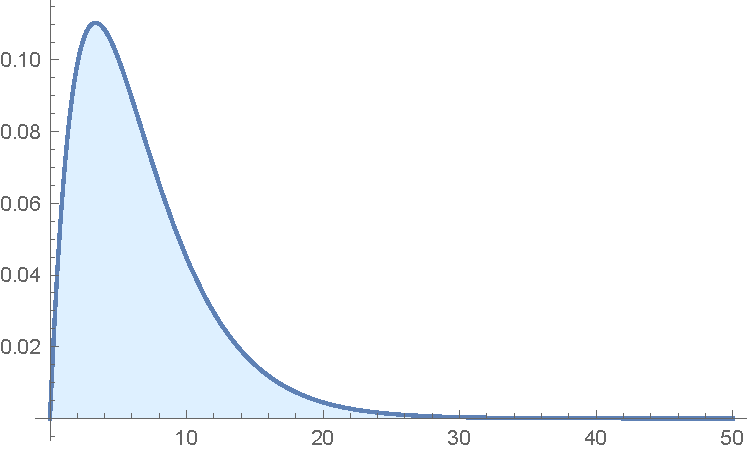
\includegraphics[width=.30\textwidth]{plot1.pdf}};
\node at(-0.7,1.5) {$PDF(t)_{A\_to\_F} * \pi_{A}$};
\node at(1.9,-0.9) {$t$};

%Plot B
\node[inner sep=0pt] at (4,0)
{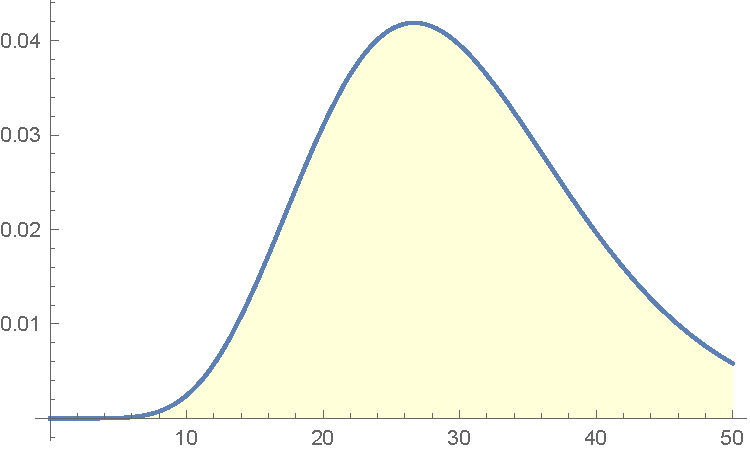
\includegraphics[width=.30\textwidth]{plot2.pdf}};
\node at(3.3,1.5) {$PDF(t)_{B\_to\_F} * \pi_{B}$};
\node at(5.9,-0.9) {$t$};

%Sum of plots
\node[inner sep=0pt] at (8,0)
{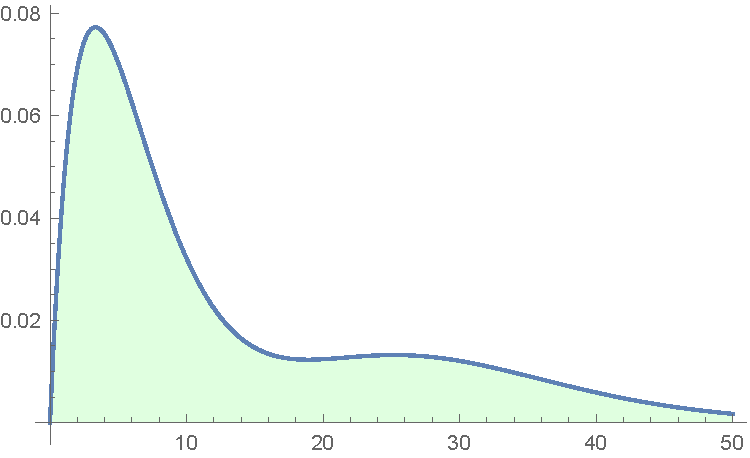
\includegraphics[width=.30\textwidth]{sumPlot.pdf}};
\node at(7.2,1.5) {$PDF(t)_{to\_F}$};
\node at(9.9,-0.9) {$t$};

%operation simbol
\draw[fill=white] (1.7,0.30) circle [radius=0.3] node {+};
\draw[fill=white] (5.7,0.30) circle [radius=0.3] node {=};
	
\end{tikzpicture}
